\documentclass[a4paper,11pt]{article}

\usepackage[english]{babel}
\usepackage[utf8x]{inputenc}
\usepackage{amsmath,amssymb,amsthm}
\usepackage{graphicx}
\usepackage{lineno}
%include the code below (between the comments) to get lineno to work better
\newcommand*\patchAmsMathEnvironmentForLineno[1]{%
  \expandafter\let\csname old#1\expandafter\endcsname\csname #1\endcsname
  \expandafter\let\csname oldend#1\expandafter\endcsname\csname end#1\endcsname
  \renewenvironment{#1}%
     {\linenomath\csname old#1\endcsname}%
     {\csname oldend#1\endcsname\endlinenomath}}% 
\newcommand*\patchBothAmsMathEnvironmentsForLineno[1]{%
  \patchAmsMathEnvironmentForLineno{#1}%
  \patchAmsMathEnvironmentForLineno{#1*}}%
\AtBeginDocument{%
\patchBothAmsMathEnvironmentsForLineno{equation}%
\patchBothAmsMathEnvironmentsForLineno{align}%
\patchBothAmsMathEnvironmentsForLineno{flalign}%
\patchBothAmsMathEnvironmentsForLineno{alignat}%
\patchBothAmsMathEnvironmentsForLineno{gather}%
\patchBothAmsMathEnvironmentsForLineno{multline}%
}
%the code is above
\linenumbers

\newtheorem{prop}{Proposition}

% Don't change the settings above. For example, the line numbers make for easy counting of the length of a piece of work.
% Don't change margins, fonts (including size) or make any other alterations which would either expand or contract the length of the resulting file. 
% You can add packages if you need but these should not impact on the length of the document, the markers have discretion to determine if such additions are appropriate. You should not need to add any packages for the first assignment.

 

\title{HCov Skills Assignment 1}
\author{Li Yueheng, s2306076}

\begin{document}
\maketitle

% What follows is poor. Make it good - see the Assignment 1 marking guide on Learn.


\section{Communication exercise} % lines formatted like this should be section headings

\begin{figure}
    \centering
    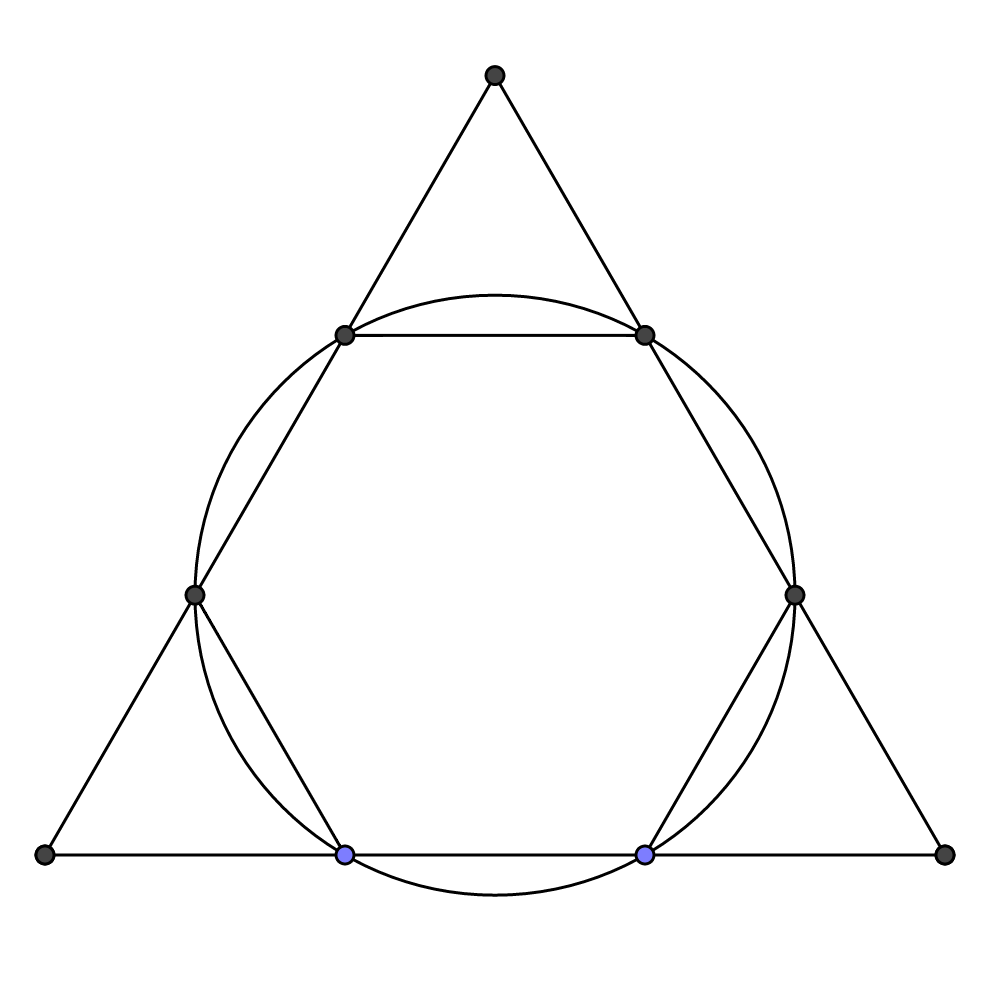
\includegraphics[width=0.4\textwidth]{d7.png}
    \caption{Caption}
\end{figure}


Replace this paragraph with your description of the figure, including a proper reference to it.


2. Holomorphic functions

\begin{prop}\label{prop:fCtoRconst} % Leave this proposition as it is.
Suppose the function \( f \) is holomorphic on \( \mathbb{C} \) and takes only real values. It follows that \( f \) must be constant.
\end{prop}

\begin{proof}
Give a clear, brief, and well-formatted proof of Proposition~\ref{prop:fCtoRconst} here. You will likely want to use the Cauchy-Riemann equations.
\end{proof}


\subsection{Microwriting}

Plagiarism is the act of copying others' work without appropriate acknowledgement or one's own previously assessed, either intentionally or unintentionally.

Collusion is a particular type of plagiarism, where students work in unauthorized collaboration in an assessed work.





% You should reference any material you use
%
%\begin{thebibliography}{9}
%
%\bibitem{Conway} 
%John B. Conway. 
%\textit{Functions of One Complex Variable I}. 
%Springer, 2010.
%
%\end{thebibliography}
%
\end{document}